% example: composite figure composed of a matplotlib and an inkscape figure (6in, 4in)
% (Tom Tetzlaff, t.tetzlaff{at}fz-juelich.de, 2020)

\documentclass{article}
\usepackage{geometry}
 \geometry{
   paperwidth=6in,
   paperheight=4in,
   top=0pt,
   bottom=0pt,
   right=0pt,
   left=0pt,
 }
\usepackage{tikz}
\usepackage{graphicx}
\pagestyle{empty}
\begin{document}
\noindent
\resizebox{\paperwidth}{!}{%
  \begin{tikzpicture}%
    %%
    \node[inner sep=-1pt] (matplotlib_figure) at (0,0)
    {\includegraphics{./matplotlib_figure.pdf}};
    %%
    \node[inner sep=-1pt,rectangle] (inkscape_sketch) at (-3.7,2.5)
    {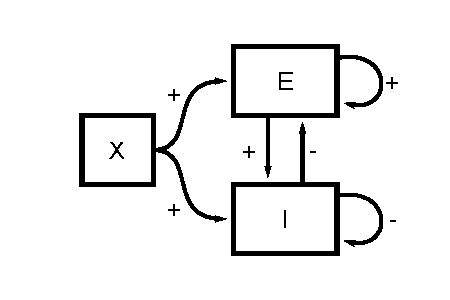
\includegraphics{./inkscape_sketch.pdf}};
    %%
    %\draw[style=help lines] (-6,-4) grid (6,4);
  \end{tikzpicture}%
}
\end{document}
